\documentclass[11pt,a4paper]{article}
\usepackage[T1]{fontenc}
\usepackage[margin=2.3cm]{geometry}
\usepackage{amsmath,amssymb}
\usepackage{graphicx}
\usepackage[dvipsnames]{xcolor}
\usepackage{enumitem}
\usepackage[colorlinks=true,linkcolor=blue,urlcolor=blue]{hyperref}
\setlength{\parskip}{0.6em}
\setlength{\parindent}{0pt}
\begin{document}

\begin{center}{\LARGE\bfseries opendistillation}\\[0.4em]{\large Separate ethanol and water with a distillation column, in three sessions.}\\[0.2em]\small PAN IIT OSS explainer \textbullet{} diploma / undergraduate to advanced undergraduate (levels 5-6)\end{center}

\section*{Why this exists}
Distillation separates mixtures by their boiling-point differences, using a column of stages. It is the workhorse of refineries, chemical plants and distilleries. This explainer follows the idea from one boil-and-condense stage to the real ethanol-water equilibrium and a McCabe-Thiele column design, using only material balances, vapour pressures and straight lines.

\section*{The end goal}
Separate ethanol and water with a distillation column: decide how many stages it needs, where the feed goes, how much reflux and steam it uses, and why no ordinary column can pass the azeotrope. The same ideas apply to crude-oil fractionation, air separation and solvent recovery.

\textit{This is a simplified educational model, not a plant design tool. Ethanol vapour is flammable; distilling alcohol needs a licence in India.}

\section*{How the three sessions build up}
\begin{enumerate}[nosep]
\item \textbf{Session 1: Boil, condense, repeat} (Level 1, conceptual interactive model, 60 min).
\item \textbf{Session 2: Real equilibrium and the azeotrope} (Level 2, mathematical engineering model, 75 min).
\item \textbf{Session 3: Design the column and validate it} (Level 3, simulation and validation, 90 min).
\end{enumerate}

\section{Session 1: Boil, condense, repeat}

\subsection*{A. Real-world problem}
A sugar-cane molasses distillery ferments a "wash" that is about 10 percent ethanol by moles (about 22 percent by mass) and 90 percent water. Ethanol boils at 78.3 C and water at 100 C, so when the wash boils the vapour carries more ethanol than the liquid. But one boil is not enough to make a strong product. How much richer is the vapour after one boil, how many boil-and-condense steps do you need to reach 80 percent ethanol, and how much of the feed comes out as product? (General education only: this is a simplified model, not a plant design method.)

\subsection*{B. Concept and theory}
We describe a mixture by \textbf{mole fractions}: x is the share of ethanol molecules in the liquid, y the share in the vapour. When a liquid boils in a closed space and settles, its vapour and liquid are in \textbf{equilibrium}, and the vapour is richer in the more volatile component (the one with the lower boiling point). The simplest model says the vapour's ethanol-to-water ratio (the "odds") is alpha times the liquid's; alpha is the \textbf{relative volatility}. Alpha = 1 means no separation; a larger alpha means an easier job. Condensing that vapour gives a new liquid that is richer still, and boiling it again enriches it more: each boil-and-condense is one \textbf{stage}, and a distillation column is a tower of stages stacked so the vapour rises and the liquid falls through them. A column splits a feed F (composition zF) into a top \textbf{distillate} D (xD) and a \textbf{bottoms} stream B (xB). Total moles and ethanol moles both balance. If all the condensed liquid at the top is sent back down (total reflux), each stage multiplies the odds by alpha, which gives the smallest possible number of stages, the \textbf{Fenske} equation.

\begin{itemize}[nosep]
\item alpha: relative volatility of ethanol to water (no unit)
\item F, D, B: feed, distillate and bottoms amounts (or flows) (mol (or kmol/h))
\item zF, xD, xB: ethanol mole fraction in feed, distillate, bottoms (no unit)
\item N\_min: minimum number of equilibrium stages (total reflux) (stages)
\end{itemize}

\begin{equation*}
y = \frac{\alpha x}{1 + (\alpha - 1)x},\qquad \frac{y}{1-y} = \alpha\,\frac{x}{1-x}
\end{equation*}

\begin{equation*}
F = D + B,\qquad F z_F = D x_D + B x_B
\end{equation*}

\begin{equation*}
D = F\,\frac{z_F - x_B}{x_D - x_B},\qquad \text{recovery} = \frac{D x_D}{F z_F}
\end{equation*}

\begin{equation*}
N_{\min} = \frac{\ln\!\left[\dfrac{x_D/(1-x_D)}{x_B/(1-x_B)}\right]}{\ln \alpha}
\end{equation*}

\begin{center}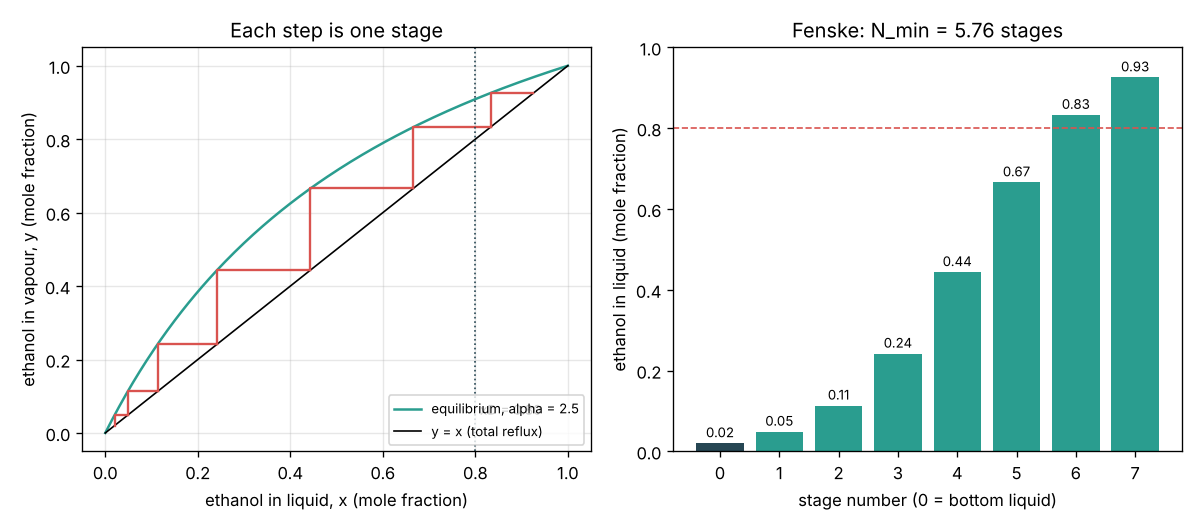
\includegraphics[width=0.85\linewidth]{figures/s01_stages_total_reflux.png}\\\small Stepping stages at total reflux from 0.02 to above 0.80 with alpha = 2.5; Fenske gives 5.76.\end{center}

\subsection*{E. Worked example}
(a) Liquid with x = 0.20 is in equilibrium with its vapour; alpha = 2.5. Find y. (b) A column takes F = 100 mol of wash with zF = 0.10 and makes xD = 0.80 and xB = 0.02. Find D, B and the ethanol recovery. (c) Find the minimum number of stages at alpha = 2.5.
\begin{enumerate}[nosep]
\item Odds in the liquid = 0.20 / 0.80 = 0.25. Odds in the vapour = 2.5 x 0.25 = 0.625, so y = 0.625 / 1.625 = 0.385 (same as 2.5 x 0.2 / (1 + 1.5 x 0.2) = 0.5 / 1.3).
\item D = 100 x (0.10 - 0.02) / (0.80 - 0.02) = 100 x 0.08 / 0.78 = 10.26 mol; B = 100 - 10.26 = 89.74 mol.
\item Check the ethanol: 10.26 x 0.80 + 89.74 x 0.02 = 8.21 + 1.79 = 10.00 mol = 100 x 0.10. It balances.
\item Recovery = 8.21 / 10.00 = 0.821: 82 percent of the ethanol leaves at the top; the rest is lost in the bottoms.
\item Odds at the top = 0.80 / 0.20 = 4; at the bottom = 0.02 / 0.98 = 0.0204. Their ratio is 196. N\_min = ln 196 / ln 2.5 = 5.278 / 0.916 = 5.76, so at least 6 whole stages.
\end{enumerate}
\textbf{Answer.} y = 0.385; D = 10.26 mol, B = 89.74 mol, recovery 0.821; N\_min = 5.76 (6 stages).

\subsection*{F. Questions}
\begin{enumerate}[nosep]
\item \textbf{Conceptual.} Why does one boil-and-condense step not give pure ethanol, even though ethanol boils 22 degrees lower than water?
\item \textbf{Numerical.} A liquid with x = 0.10 boils with alpha = 3. Find y, and check that the answer is reasonable.
\item \textbf{Graph and simulation interpretation.} In the stage figure the steps are short at the bottom, long in the middle and short again near the top. Why? What happens to the number of stages if you ask for xB = 0.01 instead of 0.02?
\item \textbf{Design and optimisation challenge.} Design: the distillery now wants xD = 0.90 and xB = 0.01 from the same 100 mol of wash (zF = 0.10, alpha = 2.5). Find N\_min, D and the recovery. What alpha would allow only 5 stages for the original job (0.80 and 0.02)?
\end{enumerate}

\section{Session 2: Real equilibrium and the azeotrope}

\subsection*{A. Real-world problem}
Session 1 treated alpha as one number. Real ethanol-water mixtures behave very differently at the dilute end and near the top: rectified spirit and fuel ethanol from a plain column stop at about 95 percent by mass, and anhydrous fuel ethanol for blending into petrol (as in India's E20 programme) needs an extra drying step. At what temperature does the wash boil, what vapour comes off, and why is there a wall that no ordinary column at atmospheric pressure can pass? (Simplified textbook model; not a plant design method.)

\subsection*{B. Concept and theory}
The \textbf{vapour pressure} Psat of a pure liquid is the pressure of its vapour in equilibrium with it; it rises steeply with temperature and is given by the Antoine equation. A liquid boils when its vapour pressure equals the pressure above it: 760 mmHg (101.325 kPa) at sea level. In an \textbf{ideal} mixture each component's partial pressure is its liquid mole fraction times its vapour pressure (\textbf{Raoult's law}). Ethanol and water are not ideal: their molecules attract their own kind more than each other, so each escapes more easily than Raoult predicts. We multiply by an \textbf{activity coefficient} gamma (here from the two-constant \textbf{van Laar} model, which gives gamma = 1 for a pure liquid and the largest gamma for a component at infinite dilution: about 5.4 for ethanol in water). The \textbf{bubble point} of a liquid x at pressure P is the temperature where the partial pressures add up to P; we find it by bisection. The vapour composition is then y = x gamma Psat / P. The local relative volatility alpha = (y / (1 - y)) / (x / (1 - x)) is about 10 for dilute ethanol and falls to 1 at the \textbf{azeotrope}, where vapour and liquid have the same composition and boiling no longer separates anything. Ethanol-water has a minimum-boiling azeotrope at about x = 0.894 and 78.15 C (measured); our model puts it at 0.915 and 78.22 C. A single equilibrium stage, a \textbf{flash}, splits a feed z into vapour V and liquid L, and the ethanol balance gives the lever rule.

\begin{itemize}[nosep]
\item A, B, C: Antoine constants (T in degrees C, P in mmHg) (as given)
\item gamma1, gamma2: activity coefficients of ethanol and water (no unit)
\item A12, A21: van Laar constants: 1.6798 and 0.9227 (no unit)
\item P, T: total pressure and temperature (mmHg, degrees C)
\item V/F: fraction of the feed that leaves as vapour in a flash (no unit)
\end{itemize}

\begin{equation*}
\log_{10} P^{\mathrm{sat}} = A - \frac{B}{T + C}
\end{equation*}

\begin{equation*}
y_i P = x_i\,\gamma_i\,P_i^{\mathrm{sat}}(T)\qquad\text{(modified Raoult's law)}
\end{equation*}

\begin{equation*}
\ln\gamma_1 = A_{12}\left(\frac{A_{21}x_2}{A_{12}x_1 + A_{21}x_2}\right)^2,\qquad \ln\gamma_2 = A_{21}\left(\frac{A_{12}x_1}{A_{12}x_1 + A_{21}x_2}\right)^2
\end{equation*}

\begin{equation*}
x_1\gamma_1 P_1^{\mathrm{sat}}(T) + x_2\gamma_2 P_2^{\mathrm{sat}}(T) = P\quad\text{(bubble point)}
\end{equation*}

\begin{equation*}
\alpha = \frac{y/(1-y)}{x/(1-x)},\qquad \frac{V}{F} = \frac{z - x}{y - x}\quad\text{(lever rule)}
\end{equation*}

\begin{center}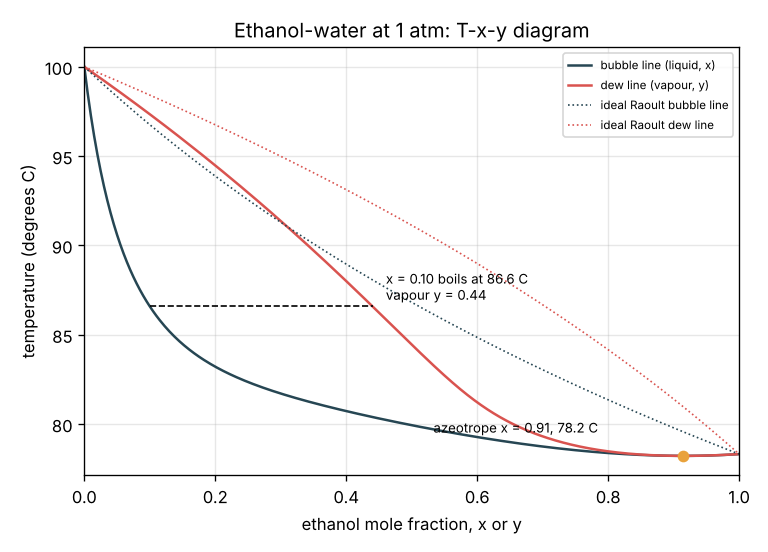
\includegraphics[width=0.85\linewidth]{figures/s02_txy.png}\\\small T-x-y diagram of ethanol-water at 1 atm with the ideal Raoult lines and the azeotrope.\end{center}

\subsection*{E. Worked example}
The wash has x = 0.10 at 760 mmHg. Find its bubble temperature, the activity coefficients, the vapour composition and the local alpha, and compare with Raoult's ideal law.
\begin{enumerate}[nosep]
\item van Laar: denominator = 1.6798 x 0.10 + 0.9227 x 0.90 = 0.998; ln gamma1 = 1.6798 x (0.8304 / 0.998)\textasciicircum{}2 = 1.163, so gamma1 = 3.197; ln gamma2 = 0.9227 x (0.168 / 0.998)\textasciicircum{}2 = 0.0261, so gamma2 = 1.027.
\item Try T = 86.6 C: Psat1 = 10\textasciicircum{}(8.20417 - 1642.89 / 316.89) = 1046.4 mmHg; Psat2 = 10\textasciicircum{}(8.07131 - 1730.63 / 320.03) = 460.6 mmHg.
\item Partial pressures: ethanol 0.10 x 3.197 x 1046.4 = 334.5 mmHg; water 0.90 x 1.027 x 460.6 = 425.5 mmHg; sum 760.0 mmHg, so 86.6 C is the bubble point.
\item y = 334.5 / 760 = 0.440. Alpha = (0.440 / 0.560) / (0.10 / 0.90) = 0.786 / 0.111 = 7.08.
\item Raoult (gamma = 1) would give a bubble point of 96.8 C and y = 0.20: the ideal model badly underestimates how easy the dilute end is.
\end{enumerate}
\textbf{Answer.} T = 86.6 C, gamma = 3.197 and 1.027, y = 0.440, alpha = 7.08 (ideal: 96.8 C, y = 0.20).

\subsection*{F. Questions}
\begin{enumerate}[nosep]
\item \textbf{Conceptual.} Why can ordinary distillation of ethanol-water at 1 atm never go beyond the azeotrope, however many stages you use?
\item \textbf{Numerical.} Find the bubble temperature and vapour composition of a liquid with x = 0.30 at 760 mmHg. Use gamma1 = 1.699, gamma2 = 1.194 and check that the partial pressures add up.
\item \textbf{Graph and simulation interpretation.} On the T-x-y diagram the gap between the bubble and dew lines is wide at x = 0.1 and nearly closed at x = 0.85. What does the width of the gap tell you, and what happens to the number of stages needed near the top of the column?
\item \textbf{Design and optimisation challenge.} Design: a one-stage still (flash) takes the wash (z = 0.10) and must give a vapour of 0.30 ethanol. Find the liquid left behind, the fraction vaporised and the temperature. Then explain whether lowering the pressure helps break the azeotrope, and at what cost.
\end{enumerate}

\section{Session 3: Design the column and validate it}

\subsection*{A. Real-world problem}
A small distillery has 100 kmol/h of fermented wash with 10 mol percent ethanol. It wants a top product of 80 mol percent ethanol (about 91 percent by mass) and wants to discard a bottom stream (stillage) with only 2 mol percent. How many stages does the column need, on which stage should the feed enter, how much liquid must be sent back down as reflux, how much steam will the reboiler use, and which reflux ratio is cheapest overall? (A simplified teaching model, not a design tool.)

\subsection*{B. Concept and theory}
A real column takes product off the top, so only part of the condensed vapour returns as reflux: the \textbf{reflux ratio} R = L / D. With \textbf{constant molar overflow} (ethanol and water have nearly equal molar latent heats, about 40 kJ/mol) the liquid L and vapour V flows are the same on every stage of a section. A mole balance around the top of the column gives the \textbf{rectifying operating line}, a straight line through (xD, xD) with slope R / (R + 1). Below the feed the liquid grows by qF and the vapour changes by (1 - q)F, giving the \textbf{stripping line} through (xB, xB); q is the liquid fraction of the feed (q = 1 for a liquid at its bubble point). The lines cross on the \textbf{q-line}. \textbf{McCabe-Thiele} stepping: start at y1 = xD (total condenser), take the liquid in equilibrium, x = x\_eq(y), then the vapour from the stage below from the operating line, and repeat; switch to the stripping line once x passes the crossing (that is the optimal \textbf{feed stage}), stop when x <= xB (the last stage is the reboiler). As R grows the operating line approaches y = x and the number of stages falls to the Fenske minimum. As R falls the line swings towards the equilibrium curve; when it touches it the steps become infinitely small: a \textbf{pinch} and the \textbf{minimum reflux} Rmin. For a 0.80 product the touch is at the feed, but because the ethanol-water curve sags towards the diagonal near the top, a higher xD touches tangentially above the feed: a \textbf{tangent pinch} with a larger Rmin. The reboiler must boil the vapour V', costing steam: duty Q = V' x latent heat. More reflux means fewer trays (capital) but more steam (energy), so there is a cheapest R, usually 1.2 to 1.5 times Rmin.

\begin{itemize}[nosep]
\item L, V: liquid and vapour flows above the feed (kmol/h)
\item L', V': liquid and vapour flows below the feed (kmol/h)
\item q: liquid fraction of the feed (1 = saturated liquid) (no unit)
\item Rmin: minimum reflux ratio (pinch, infinite stages) (no unit)
\item Q\_R: reboiler duty V' x 40 kJ/mol (kW)
\item E: overall tray efficiency (real trays = stages / E) (no unit)
\end{itemize}

\begin{equation*}
y_{n+1} = \frac{R}{R+1}\,x_n + \frac{x_D}{R+1}\quad\text{(rectifying line)}
\end{equation*}

\begin{equation*}
y_{m+1} = \frac{L'}{V'}\,x_m - \frac{B\,x_B}{V'},\qquad L' = L + qF,\quad V' = V - (1-q)F
\end{equation*}

\begin{equation*}
y = \frac{q}{q-1}\,x - \frac{z_F}{q-1}\quad\text{(q-line; } x = z_F \text{ for } q = 1)
\end{equation*}

\begin{equation*}
R_{\min} = \frac{x_D - y^*}{y^* - x^*}\quad\text{at the pinch point } (x^*, y^*)
\end{equation*}

\begin{equation*}
Q_R = V'\,\lambda,\qquad \text{cost} = c_{\mathrm{tray}}\,\left\lceil \frac{N-1}{E} \right\rceil + c_{\mathrm{steam}}\,Q_R
\end{equation*}

\begin{center}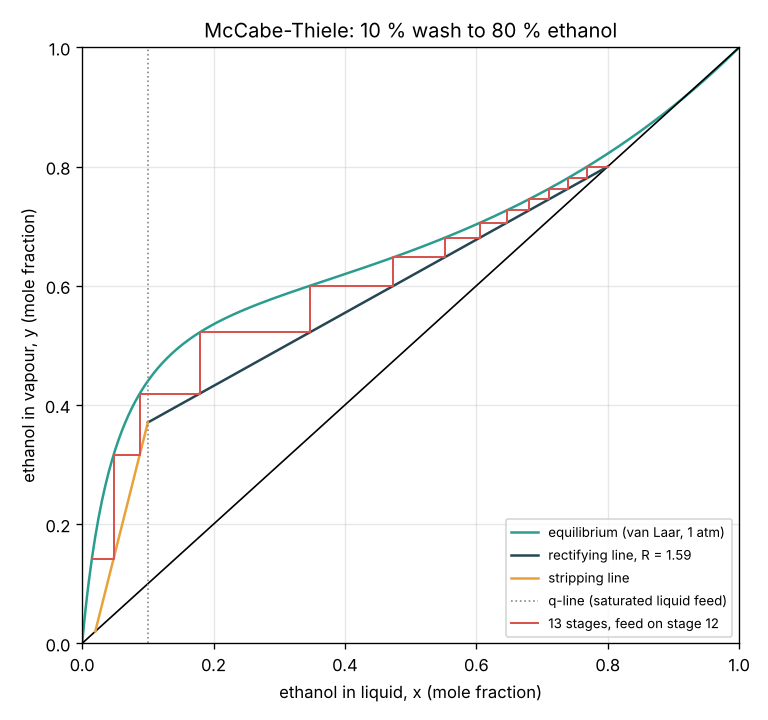
\includegraphics[width=0.85\linewidth]{figures/s03_mccabe_thiele.png}\\\small McCabe-Thiele diagram: 13 stages, feed on stage 12, for a 10 \% wash to 80 \% ethanol.\end{center}

\subsection*{E. Worked example}
Design the distillery column: F = 100 kmol/h, zF = 0.10 (saturated liquid), xD = 0.80, xB = 0.02, 1 atm. Find Rmin, the stages and feed stage at R = 1.5 Rmin, and the reboiler duty.
\begin{enumerate}[nosep]
\item Material balance (Session 1): D = 100 x 0.08 / 0.78 = 10.26 kmol/h, B = 89.74 kmol/h.
\item Pinch at the feed: the wash's vapour (Session 2) is y* = 0.440, so Rmin = (0.80 - 0.440) / (0.440 - 0.10) = 1.058. (A scan over all x from 0.10 to 0.80 confirms the feed point is the tightest.)
\item R = 1.5 x 1.058 = 1.587. Rectifying line: y = 0.6135 x + 0.3092. L = 16.28, V = 26.53 kmol/h; with q = 1, L' = 116.28 and V' = 26.53 kmol/h.
\item Step from the top: x1 = 0.769, x2 = 0.739, ... x11 = 0.088 crosses zF, so stage 12 is the feed stage; x12 = 0.048, x13 = 0.015 <= 0.02. 13 stages including the reboiler, so 12 trays in theory, 20 real trays at 60 percent efficiency.
\item Reboiler duty = 26.53 kmol/h x 40 kJ/mol x 1000 / 3600 = 294.8 kW.
\end{enumerate}
\textbf{Answer.} Rmin = 1.058; at R = 1.587 the column needs 13 stages (12 theoretical trays plus the reboiler, 20 real trays), feed on stage 12, reboiler duty 295 kW.

\subsection*{F. Questions}
\begin{enumerate}[nosep]
\item \textbf{Conceptual.} Why does the column need more and more stages as the reflux ratio approaches Rmin, and why can it not run below Rmin at all?
\item \textbf{Numerical.} For the same column at R = 1.5 Rmin = 1.587, find L, V, L' and V' in kmol/h. Check that V' = L' - B and that the two operating lines meet at x = zF = 0.10.
\item \textbf{Graph and simulation interpretation.} In the trade-off figure the number of stages falls in steps while the duty rises smoothly, and the cost curve is jagged. Why? Why does the cost rise sharply below about 1.2 Rmin?
\item \textbf{Design and optimisation challenge.} Design: a richer wash with zF = 0.20 arrives (same xD = 0.80, xB = 0.02, 100 kmol/h). The hand formula with y* = y\_eq(0.20) = 0.535 gives Rmin = 0.789. Use \texttt{min\_reflux} to check it, then design at 1.5 Rmin. What changes, and why?
\end{enumerate}

\section{Real-world mini-project}
\textbf{Choose the reflux ratio of a distillery column.} The distillery column of Section E has to be built and run for years. Each real tray costs 2.0 lakh rupees per year (build cost spread over its life) and each kW of reboiler steam costs 0.24 lakh rupees per year. The tray efficiency is 0.6. Use \texttt{design} from Session 3 for reflux ratios from 1.05 to 3.0 times Rmin in steps of 0.05. These costs are illustrative numbers, not quotes.

\section{The path ahead}
\begin{enumerate}[nosep]
\item \textbf{Session 4: Energy balances on every tray.} A stage-by-stage calculation with an enthalpy balance on every tray, so L and V change down the column, using liquid and vapour enthalpies from simple heat-capacity and latent-heat data.
\item \textbf{Session 5: Tray efficiency and real trays.} McCabe-Thiele stepping to a "pseudo-equilibrium" curve y = y\_op + E\_MV (y\_eq - y\_op), and a comparison with the overall efficiency of Session 3.
\item \textbf{Session 6: Breaking the azeotrope.} A material and energy balance for a column making near-azeotrope ethanol followed by a molecular-sieve dryer, and a T-x-y study of how the azeotrope moves with pressure.
\item \textbf{Session 7: A dynamic column.} Tray hold-ups and component balances dM x / dt = in - out on every stage, integrated in time from a cold, uniform start, with a simple liquid-flow (weir) relation.
\item \textbf{Session 8: Controlling the column.} A PI loop that adjusts the reflux ratio to hold the temperature of a sensitive tray, tested on the dynamic column of Session 7.
\end{enumerate}

\section{Answers and hints}

\subsection*{Session 1}
\begin{enumerate}[nosep]
\item \textbf{Conceptual.} Hint: At the boiling temperature of the mixture, does water have zero vapour pressure? Solution: At the mixture's boiling point both liquids have a vapour pressure, so both evaporate. The vapour is richer in ethanol (alpha is above 1) but still contains water. The odds improve by a factor alpha per stage, never by an infinite factor, so pure ethanol would need infinitely many stages even without the azeotrope of Session 2.
\item \textbf{Numerical.} Hint: y = alpha x / (1 + (alpha - 1) x). Solution: y = 3 x 0.10 / (1 + 2 x 0.10) = 0.30 / 1.20 = 0.25. Check: y is above x (enrichment) and below 1; the odds go from 0.111 to 0.333, a factor of 3 = alpha.
\item \textbf{Graph and simulation interpretation.} Hint: Each stage multiplies the odds by the same factor; how big is a fixed change in odds near x = 0 or x = 1? Solution: A constant factor on the odds is a small change in x when x is close to 0 or 1 and a large change near x = 0.5, because the odds curve x / (1 - x) is steep only near the ends. Halving xB doubles the odds ratio (196 to about 396), adding ln 2 / ln 2.5 = 0.76 stage: N\_min goes from 5.76 to 6.53, so 7 whole stages.
\item \textbf{Design and optimisation challenge.} Hint: Use min\_stages and split; for alpha, solve ln 196 / ln alpha = 5. Solution: N\_min = ln[(0.9 / 0.1) / (0.01 / 0.99)] / ln 2.5 = ln 891 / 0.916 = 7.41, so 8 stages. D = 100 x 0.09 / 0.89 = 10.11 mol; recovery = 10.11 x 0.90 / 10 = 0.910. For 5 stages, alpha = 196\textasciicircum{}(1/5) = 2.87. Trade-off: purer products and better recovery cost stages; and at total reflux there is no product at all, so a real column needs more than N\_min (Session 3).
\end{enumerate}

\subsection*{Session 2}
\begin{enumerate}[nosep]
\item \textbf{Conceptual.} Hint: What is y - x at the azeotrope, and what does a stage do if y = x? Solution: A stage enriches the liquid only because its vapour is richer (y > x). At the azeotrope y = x, so condensing the vapour gives back exactly the same liquid: alpha = 1 and the stage does nothing. Approaching from below, the steps get smaller and smaller, so infinitely many stages would be needed even to reach it. Above it, the vapour is poorer than the liquid. To pass it you need another method: a pressure change, an entrainer (azeotropic distillation) or molecular-sieve drying.
\item \textbf{Numerical.} Hint: Try T = 81.7 C: compute both vapour pressures with Antoine. Solution: At 81.7 C: Psat1 = 868.3 mmHg and Psat2 = 379.8 mmHg. Ethanol: 0.30 x 1.699 x 868.3 = 442.6 mmHg; water: 0.70 x 1.194 x 379.8 = 317.4 mmHg; total 760.0 mmHg, so T = 81.7 C. y = 442.6 / 760 = 0.582. Alpha = (0.582 / 0.418) / (0.30 / 0.70) = 3.25: still a good separation, but well below the 7.08 of the wash.
\item \textbf{Graph and simulation interpretation.} Hint: The tie line runs from the bubble line to the dew line at one temperature. Solution: The gap is y - x, the enrichment one stage gives. At x = 0.1 the vapour is 0.44, a jump of 0.34; at x = 0.85 alpha is 1.08 and y - x is only about 0.01. So the top of an ethanol column needs many stages for small gains, and the curve's closeness to the diagonal there is what limits how high xD can be set (Session 3).
\item \textbf{Design and optimisation challenge.} Hint: Find x where y(x) = 0.30 (use flash\_from\_liquid in a small loop), then V/F = (z - x) / (y - x). Use azeotrope(p) at lower pressures. Solution: Bisection gives x = 0.0436 at 91.4 C, and V/F = (0.10 - 0.0436) / (0.30 - 0.0436) = 0.220: 22 percent of the feed boils off. In the model the azeotrope moves from x = 0.915 at 760 mmHg to 0.933 at 400 mmHg and 0.972 at 100 mmHg; measurements show the same trend and that it disappears only at very low pressure (roughly 10 kPa or below). Trade-off: vacuum lowers the temperatures and shifts the wall, but needs very large columns (vapour volume grows as pressure falls), a vacuum system and cold cooling water, so industry usually uses molecular sieves or an entrainer instead. The vacuum numbers are from a simplified model.
\end{enumerate}

\subsection*{Session 3}
\begin{enumerate}[nosep]
\item \textbf{Conceptual.} Hint: What happens to the size of a step where the operating line meets the equilibrium curve? Solution: Each step lives between the operating line and the equilibrium curve. As R falls, the rectifying line rises towards the curve, the gap shrinks and the steps get shorter, so more of them are needed. At Rmin the line touches the curve: near the touching point the steps become infinitely small (a pinch), so infinitely many stages are needed. Below Rmin the line would cross the curve and the staircase cannot get past the crossing: the separation is impossible at any number of stages.
\item \textbf{Numerical.} Hint: L = R D, V = L + D, L' = L + F, V' = V for q = 1. Solution: D = 10.26, L = 1.587 x 10.26 = 16.28, V = 26.53 kmol/h. L' = 16.28 + 100 = 116.28, V' = 26.53 kmol/h, and L' - B = 116.28 - 89.74 = 26.53 = V'. At x = 0.10 the rectifying line gives 0.6135 x 0.10 + 0.3092 = 0.3706; the stripping line gives (116.28 / 26.53) x 0.10 - (89.74 x 0.02) / 26.53 = 0.4383 - 0.0677 = 0.3706. They meet on the q-line, as they must.
\item \textbf{Graph and simulation interpretation.} Hint: Stages are whole numbers; duty is (R + 1) D times the latent heat. Solution: You cannot build 12.4 stages, so the stage count jumps by whole stages while the duty, (R + 1) x 10.26 kmol/h x 40 kJ/mol, rises in a straight line. The cost adds a staircase to a straight line, so it is jagged. Near Rmin the stage count explodes (23 stages at 1.1 Rmin, infinite at Rmin) while the duty saves only a little, so the tray cost dominates and the total rises steeply.
\item \textbf{Design and optimisation challenge.} Hint: min\_reflux scans every x between zF and xD; compare where it finds the pinch. Solution: \texttt{min\_reflux(0.20, 0.80)} gives Rmin = 0.942 with the pinch at x = 0.597: a tangent pinch above the feed, so the feed-point formula (0.789) would under-design the column. At R = 1.5 x 0.942 = 1.413 the column needs 14 stages with the feed on stage 13; D = 23.08 kmol/h and the reboiler duty is 619 kW, about twice as much because twice as much ethanol is distilled. Trade-off: always check the whole curve for a tangent pinch with ethanol-water; and a product above about 0.89 is impossible however you design it, because of the azeotrope. All costs and efficiencies are illustrative.
\end{enumerate}

\section{How to join}
Read \texttt{CONTRIBUTING.md} in the repository, then pick an issue labelled \texttt{good first issue}. Repository: \url{https://github.com/KrunalPanchal1995/pan-iit-oss/tree/main/opendistillation}

\end{document}
